\documentclass[
11pt,%
tightenlines,%
twoside,%
onecolumn,%
nofloats,%
nobibnotes,%
nofootinbib,%
superscriptaddress,%
noshowpacs,%
centertags]%
{revtex4}
\usepackage{ljm}
\usepackage{listings}
\usepackage{amsmath}

\lstset{
language=C++,
basewidth=0.5em,
xleftmargin=45pt,
xrightmargin=45pt,
basicstyle=\small\ttfamily,
keywordstyle=\bfseries\underbar,
numbers=left,
numberstyle=\tiny,
stepnumber=1,
numbersep=10pt,
showspaces=false,
showstringspaces=false,
showtabs=false,
frame=trBL,
tabsize=2,
captionpos=t,
breaklines=true,
breakatwhitespace=false,
escapeinside={\%*}{*)}
}

\begin{document}

\titlerunning{solving nonlinear equations}
\authorrunning{Bagrov, Rybakov}

\title{Selection of a method for solving nonlinear equations in shallow-water icing model implementation}

\author{\firstname{A.~D.}~\surname{Bagrov}}
\email[E-mail: ]{andrey.bagrov@yandex.ru}
\affiliation{Joint Supercomputer Center of the Russian Academy of Sciences -- branch of Scientific Research Institute of System Analysis of the Russian Academy of Sciences, Leninsky prospect 32a, Moscow, 119334, Russia}

\author{\firstname{A.~A.}~\surname{Rybakov}}
\email[E-mail: ]{rybakov.aax@gmail.com}
\affiliation{Joint Supercomputer Center of the Russian Academy of Sciences -- branch of Scientific Research Institute of System Analysis of the Russian Academy of Sciences, Leninsky prospect 32a, Moscow, 119334, Russia}

\firstcollaboration{(Submitted by TODO)} % Add if you know submitter.
%\lastcollaboration{ }

\received{TODO}

\begin{abstract}
Ice accretion simulation on aircraft profiles during their flight in an air stream containing supercooled water droplets is an extremely important task for flight safety, since the form of accreted ice significantly affects flight characteristics.
In one of the models for solving the problem, the shallow-water icing model (SWIM), the problem of solving nonlinear equations with one variable plays a central role in numerical simulation.
Since this problem occupies the overwhelming majority of calculations time, the question of choosing the optimal method for solving nonlinear equations and optimizing these methods becomes especially acute.
This article describes the analysis of the use of various methods for solving nonlinear equations in the implementation of the SWIM solver, taking into account the features of the equations being solved, which led to a significant acceleration of the computational codes when performing calculations on JSCC RAS supercomputers.
\end{abstract}

\subclass{65H05, 65Y20} % Enter 2010 Mathematics Subject Classification.

\keywords{nonlinear equations, shallow-water icing model, bisection method, Newton's method, Brent's method}

\maketitle

\section{Introduction}

At present, there are a lot of computational codes used for numerical simulation of icing on a streamlined body surface.
Some of the most popular packages for this task are Lewice \cite{Wright} and ONERA.
In this article, we will not discuss the features of these calculation packages and the differences between them, but consider only the implementation of the SWIM solver, described in detail in \cite{Bourgault}.
When performing computer simulation of the icing process of a surface in a free stream, the shallow-water icing model performs a simultaneous calculation of the ice accretion and the flow of a liquid film over the surface of the streamlined body. This takes into account the loss of moisture on the surface of the body, evaporation of water or sublimation of ice from the surface of the body, the flow of a liquid film over the surface with its partial freezing, as well as the overflow of heat fluxes between the body and the surface and between the surface and the surrounding air.

Numerical calculations are performed on a surface computational mesh, consisting of individual cells, while in each cell of the surface, the mass conservation law must be fulfilled, written in the following form:

\begin{equation}
\rho_w \left[ \frac{\partial h_f}{\partial t} + \operatorname{div}(\overline{u} h_f) \right] = U_{\infty} LWC \beta - \dot m_{evap} - \dot m_{ice}
\end{equation}

In this formula, $\rho_w$ is the density of water, $h_f$ is the height of the water film on the surface, $\overline{u}$ is the velocity of the water film, $U_{\infty}$ is the speed of the free stream, $LWC$ is the liquid water content in the free stream, $\dot m_{evap}$ is the specific rate of evaporation or sublimation from the surface of the streamlined body, $\dot m_{ice}$ is the specific rate of ice mass increasing.

In addition, the law of conservation of energy is fulfilled in each cell:

\begin{equation}
\begin{aligned}
& \rho_w \left[ \frac{\partial h_f C_w \tilde{T}}{\partial t} + \operatorname{div}(\overline{u} h_f C_w \tilde{T}) \right] = \left[ C_w \tilde{T}_{d,\infty} + \frac{||\overline{u}_d||^2}{2} \right] \times U_{\infty} LWC \beta
\\
& - \frac{1}{2}(L_{evap} + L_{subl}) \dot m_{evap} + (L_{fusion} - C_{ice} \tilde{T}) \dot m_{ice} + \sigma (T_{\infty}^4 - T^4) + \dot Q_h + \dot Q_{cond}
\end{aligned}
\end{equation}

In this formula, $C_w$ is the specific heat of water, $\tilde{T}$ is the cell temperature in degrees Celsius, $\tilde{T}_{d,\infty}$ is the temperature of the inpingement droplets in degrees Celsius, $\overline{u}_d$ is the speed of droplets falling onto the surface, $L_{evap}$ is the latent heat of water evaporation, $L_{subl}$ is the latent heat of ice sublimation, $L_{fusion}$ is the latent the heat of ice melting, $C_{ice}$ is the heat capacity of ice, $\sigma$ is the Boltzmann constant, $T_{\infty}$ is the free stream temperature in kelvin, $T$ is the cell temperature in kelvin, $\dot Q_h$ is the specific value of the heat flux received from the air, $\dot Q_{cond}$ is the specific value of the heat flux entering the cell from the surface.

For the numerical solution of the given system of equations, it is necessary to discretize it in time and space, as shown in \cite{Beaugendre}.
After that, we obtain a system of two difference equations, which include three unknown variables: surface temperature $\tilde{T}$, height of water film $h_f$ and height of ice $h_{ice}$.

Also, when solving the system of equations, the compatibility conditions must be satisfied, written in the form

\begin{equation}
\begin{cases}
h_f \ge 0\\
\dot m_{ice} \ge 0\\
h_f \tilde{T} \ge 0\\
\dot m_{ice} \tilde{T} \le 0
\end{cases}
\end{equation}

\begin{figure}[h]
\setcaptionmargin{5mm}
\onelinecaptionstrue
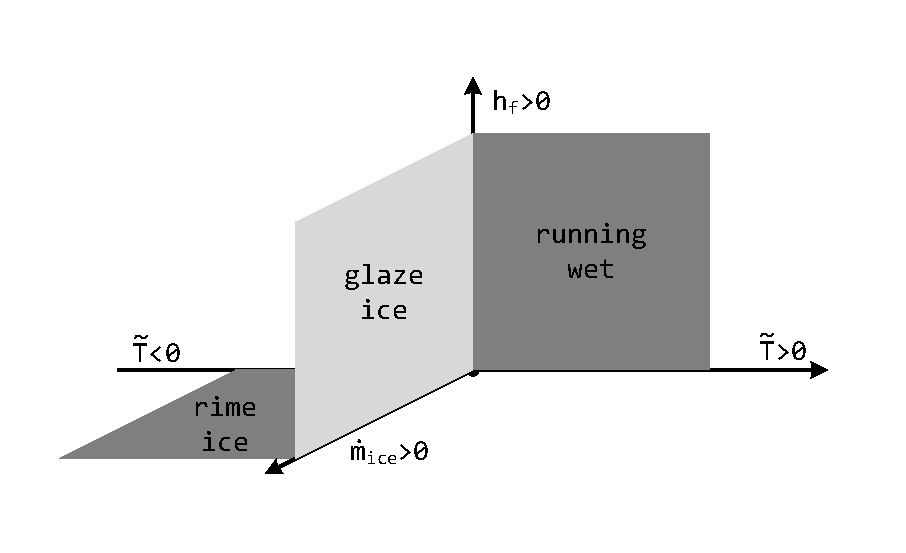
\includegraphics[width=0.7\textwidth]{pics/surface.pdf}
\captionstyle{normal}\caption{The space of solutions of the system of equations for the mass and heat balance of the cell.}\label{fig:surface}
\end{figure}

Despite the fact that there are more unknowns in the equation than the equations themselves, the system is still solved, since these variables are not completely independent.
The solution is taken from the condition that the cell can be in one of three states.
The first state is running wet, it is reached when there is no ice in the cell and a liquid film flows.
In this case, the temperature cannot be negative.
The second state is glaze icing, if both ice and water are present in the cell at the same time.
In this case, the temperature is zero degrees Celsius.
And finally, in the third case, at a negative temperature, the cell cannot contain water and only ice is present.
The general solution space is shown in Fig.~\ref{fig:surface}.

\section{Features of the equations being solved}

For glaze ice state of the cell the system of equations consisting of the mass balance equation and the heat balance equation degenerates into a simple system of linear equations with two unknown variables (the height of the water film and the height of the ice).
The solution of such a system of equations is not difficult.
For the two remaining states of the cell (running wet, rime ice), the described system of equations is reduced to one nonlinear equation with one variable (the unknown variable in this case is the cell temperature).
In this case, the nonlinear equation includes such physical essences as the specific heat of water, ice and air ($C_w$, $C_{ice}$, $C_a$), the latent heat of evaporation and sublimation ($L_{ev}$, $L_su$), as well as the dynamic viscosity of water ($\mu_w$).
These values are not constants, but they themselves depend on temperature in a nonlinear manner.
Fig.~\ref{fig:ph_graphics_h} shows piecewise-linear interpolation of these physical essences, performed according to their tabular values.

\begin{figure}[h]
\setcaptionmargin{5mm}
\onelinecaptionstrue
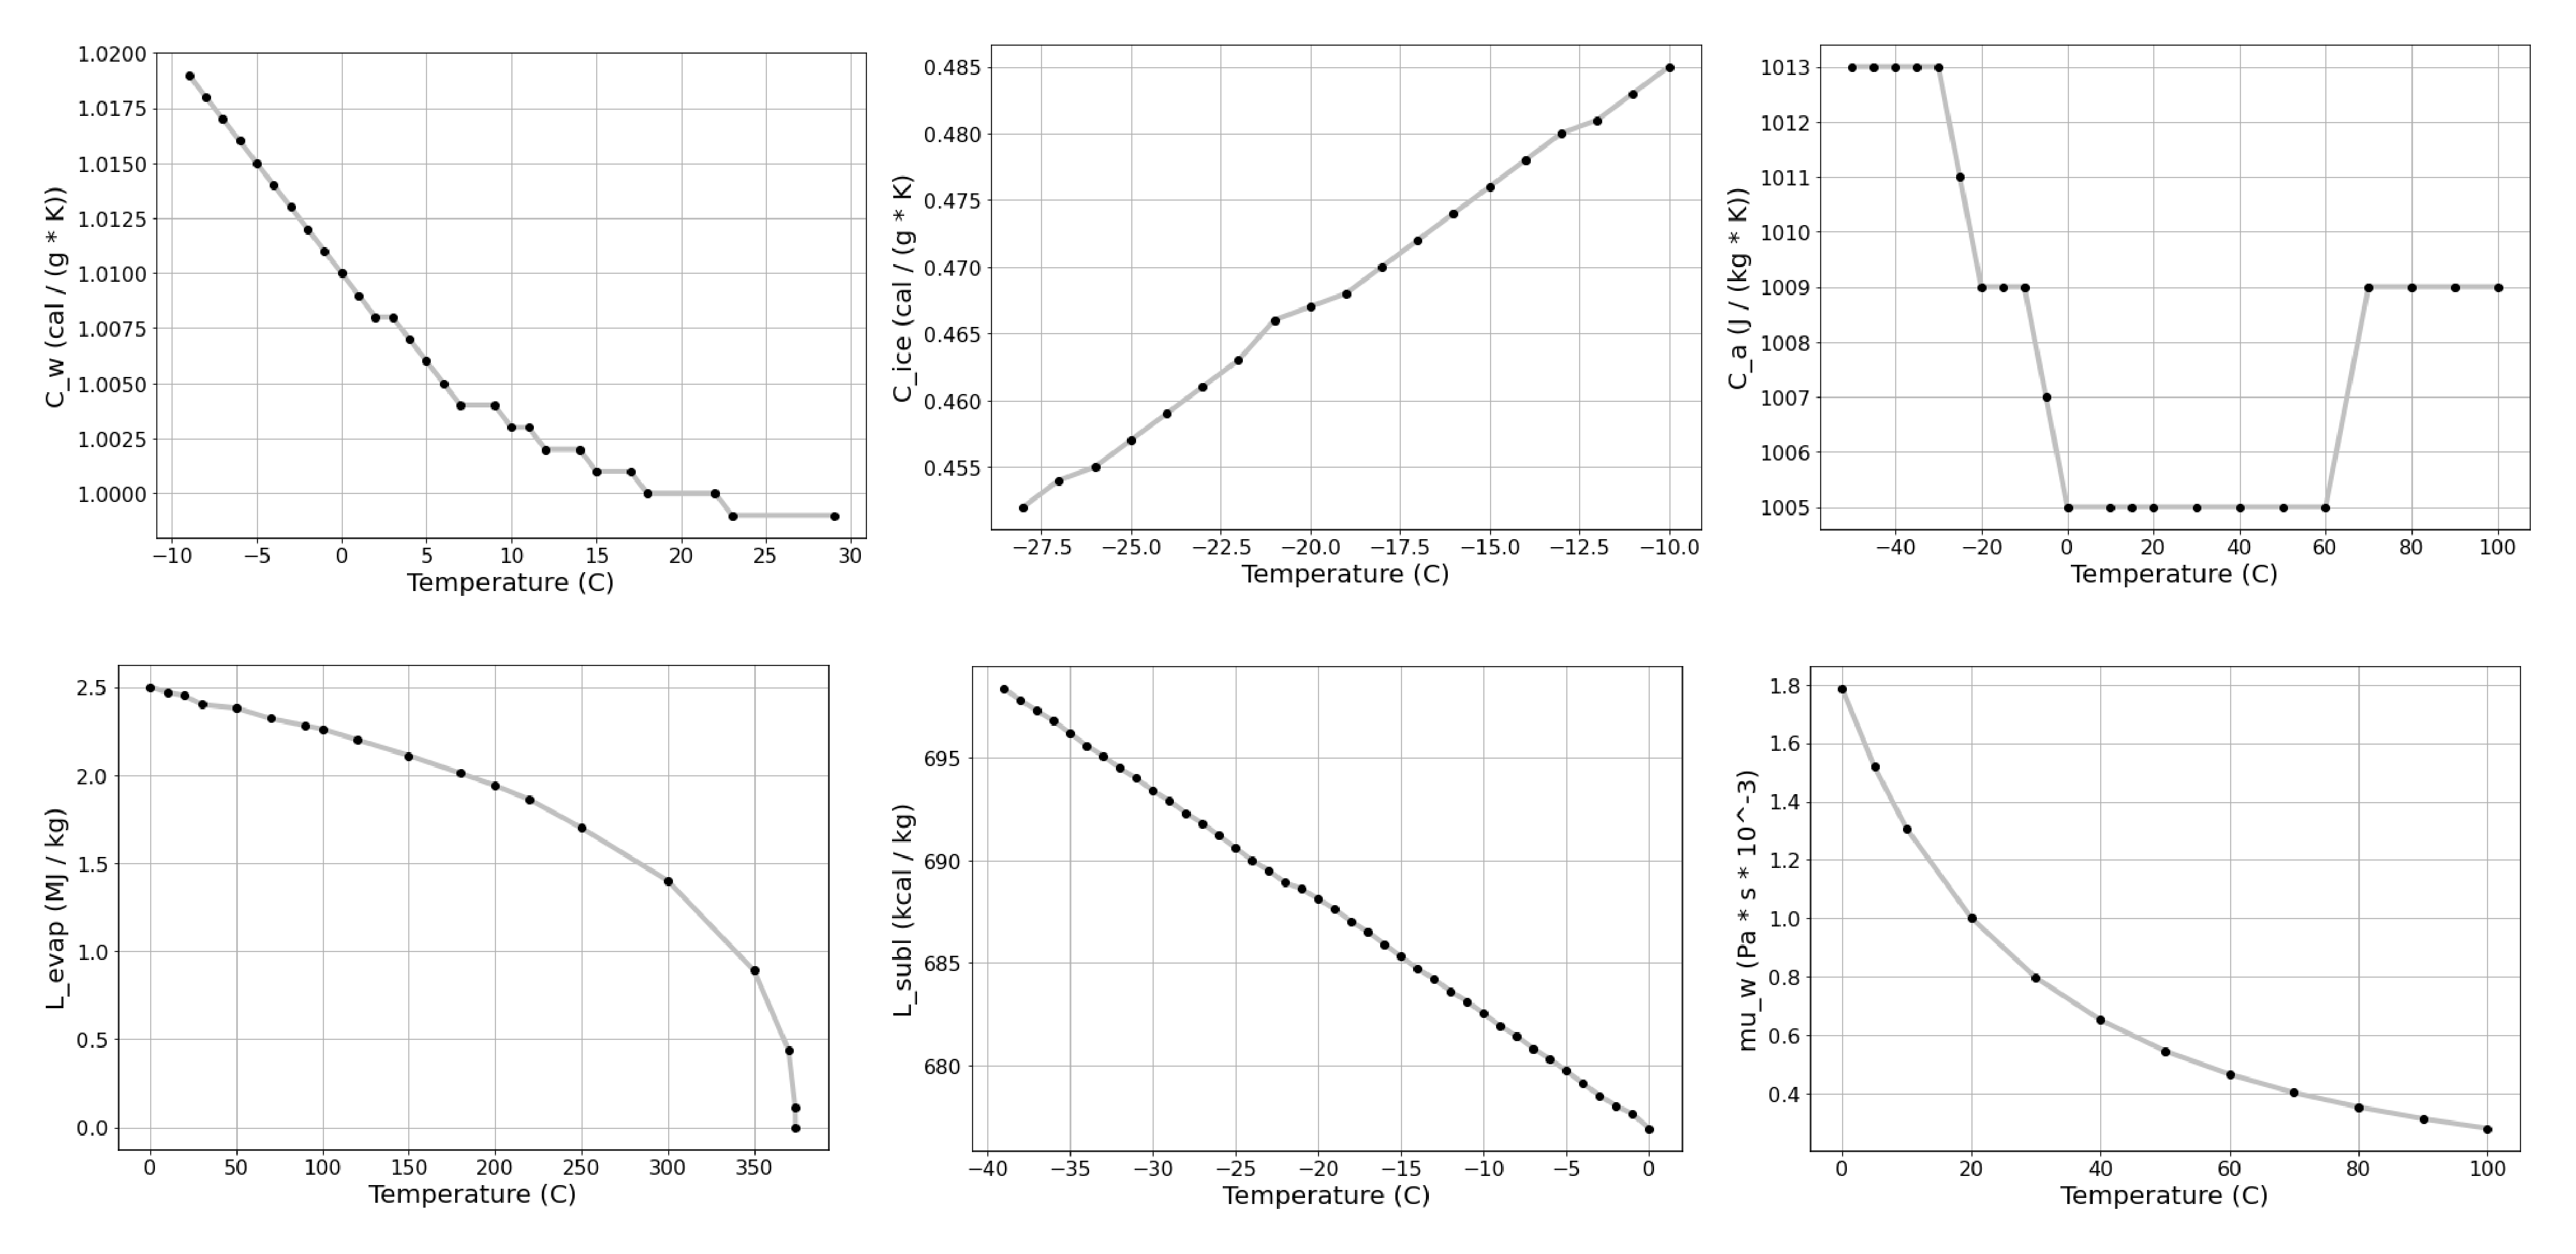
\includegraphics[width=1.0\textwidth]{pics/ph_graphics_h.pdf}
\captionstyle{normal}\caption{Dependences of physical values on temperature.}\label{fig:ph_graphics_h}
\end{figure}

In the process of performing calculations on a scale of the entire surface, unstructured computational meshes with a characteristic number of cells $10^5 $ were used, the characteristic computation time is $10^3$ seconds, and the characteristic time step is $10^{-3}$ seconds.
In the general case, at each time step, it is required to solve the nonlinear equation from 0 to 2 times (we will assume that, on average, 1 time).
In total, we find that the typical number of launches of solving a nonlinear equation in the process of starting a typical computational problem is $10^11$ calls.
This number of launches of solving nonlinear equations is essential even if computations are parallelized using MPI, OpenMP, and vectorization of the program code.
Therefore, the choice of the optimal method for solving nonlinear equations is a critical task for increasing the speed of the program code.

When testing various methods for solving nonlinear equations, the profiles of the functions ($f(x)$) were collected, for which it is required to find a solution.
The variety of these profiles is shown in Fig.~\ref{fig:dq}.
This illustration plots the family of functions $f(x)$ for randomly selected cells of the computational mesh for random times and for resolving various states of the cells.

\begin{figure}[h]
\setcaptionmargin{5mm}
\onelinecaptionstrue
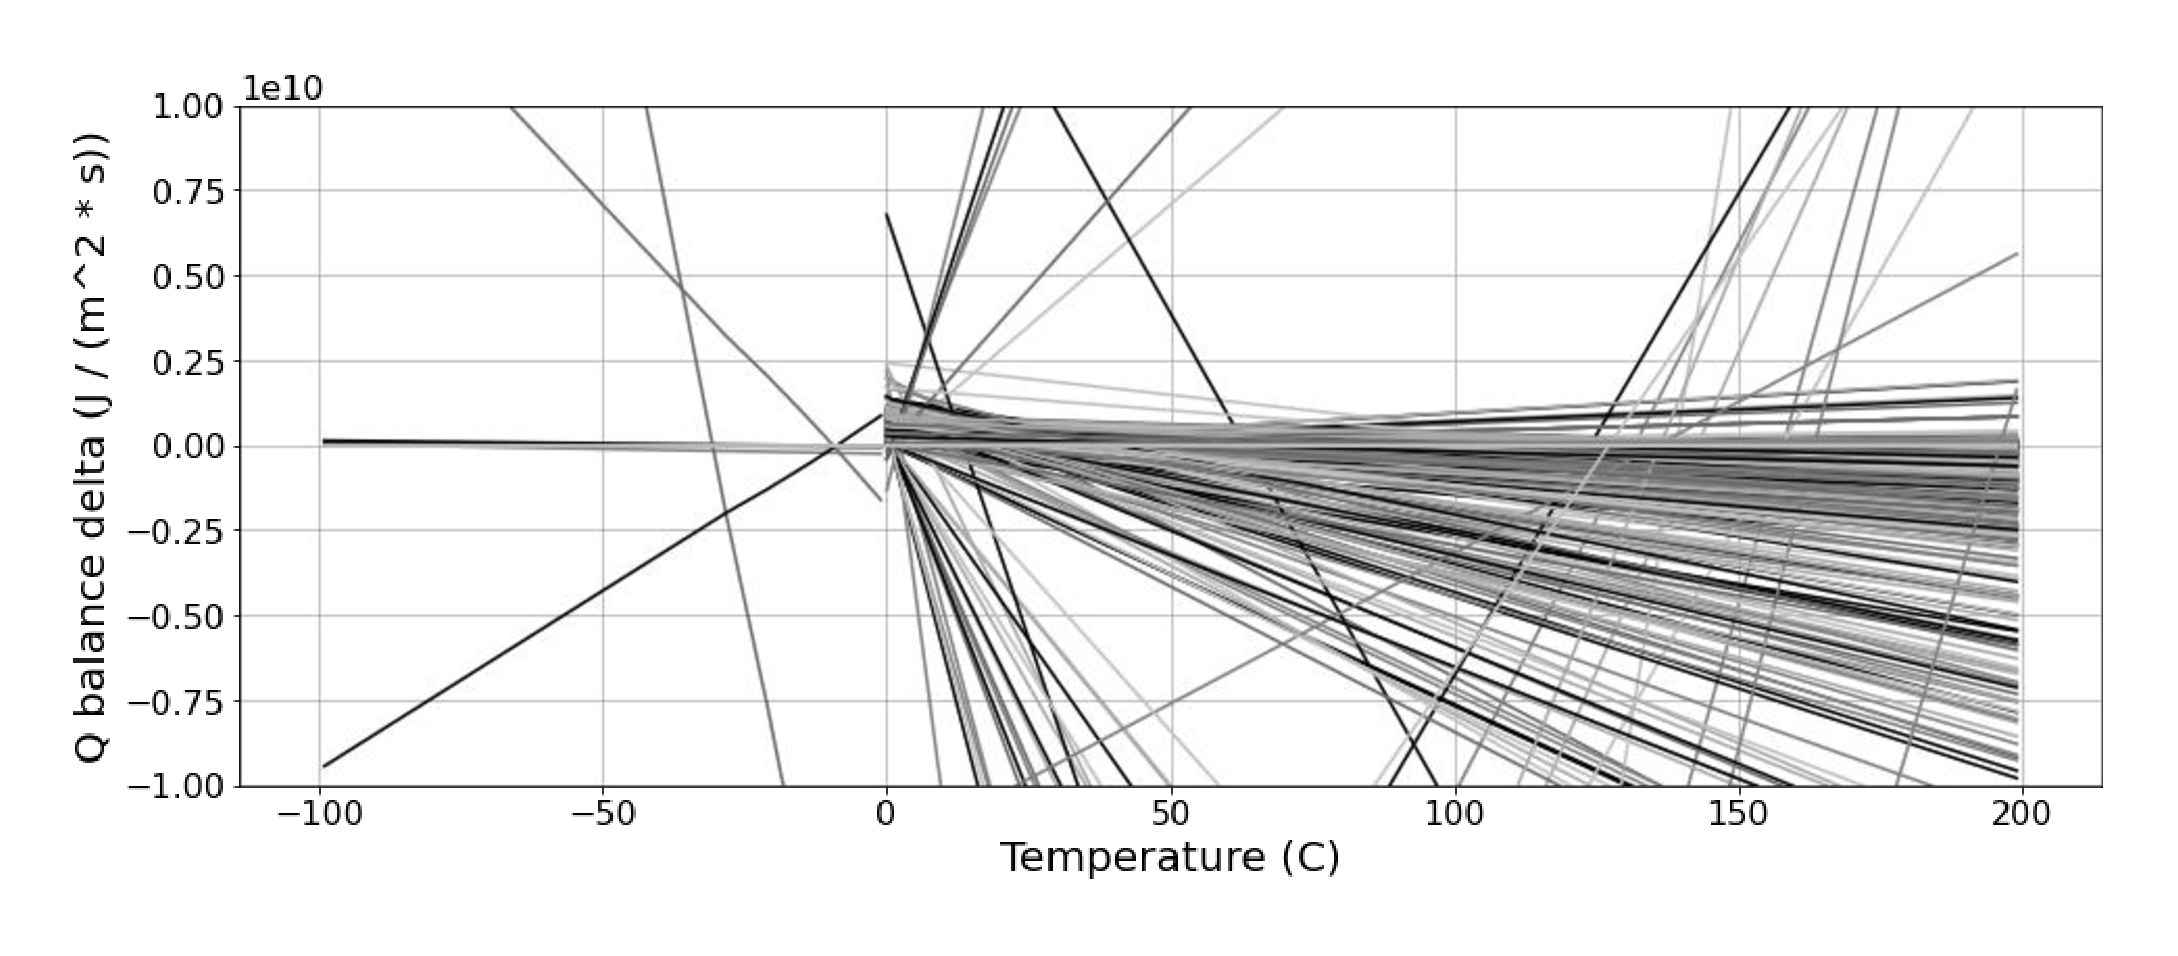
\includegraphics[width=1.0\textwidth]{pics/dq.pdf}
\captionstyle{normal}\caption{Graphs of functions representing nonlinear equations to be solved.}\label{fig:dq}
\end{figure}

From the given illustration, one might get the impression that the equations were mainly solved for the states of the cell running wet (since the plotting area $x > 0$ is densely filled with plots).
However, this impression is erroneous, just most of the graphs of the $f(x)$ functions for the state of the rime ice cell at a given scale are strongly pressed from the $OX$ axis and merge into one graph.
Fig.~\ref{fig:dq_rime_wet} shows graphs of functions for resolving the states of cells rime ice (left) and running wet (right) separately and on different scales.
In these graphs, you can observe the general view of the graphs representing the equations for resolving these two states of the cell.

\begin{figure}[h]
\setcaptionmargin{5mm}
\onelinecaptionstrue
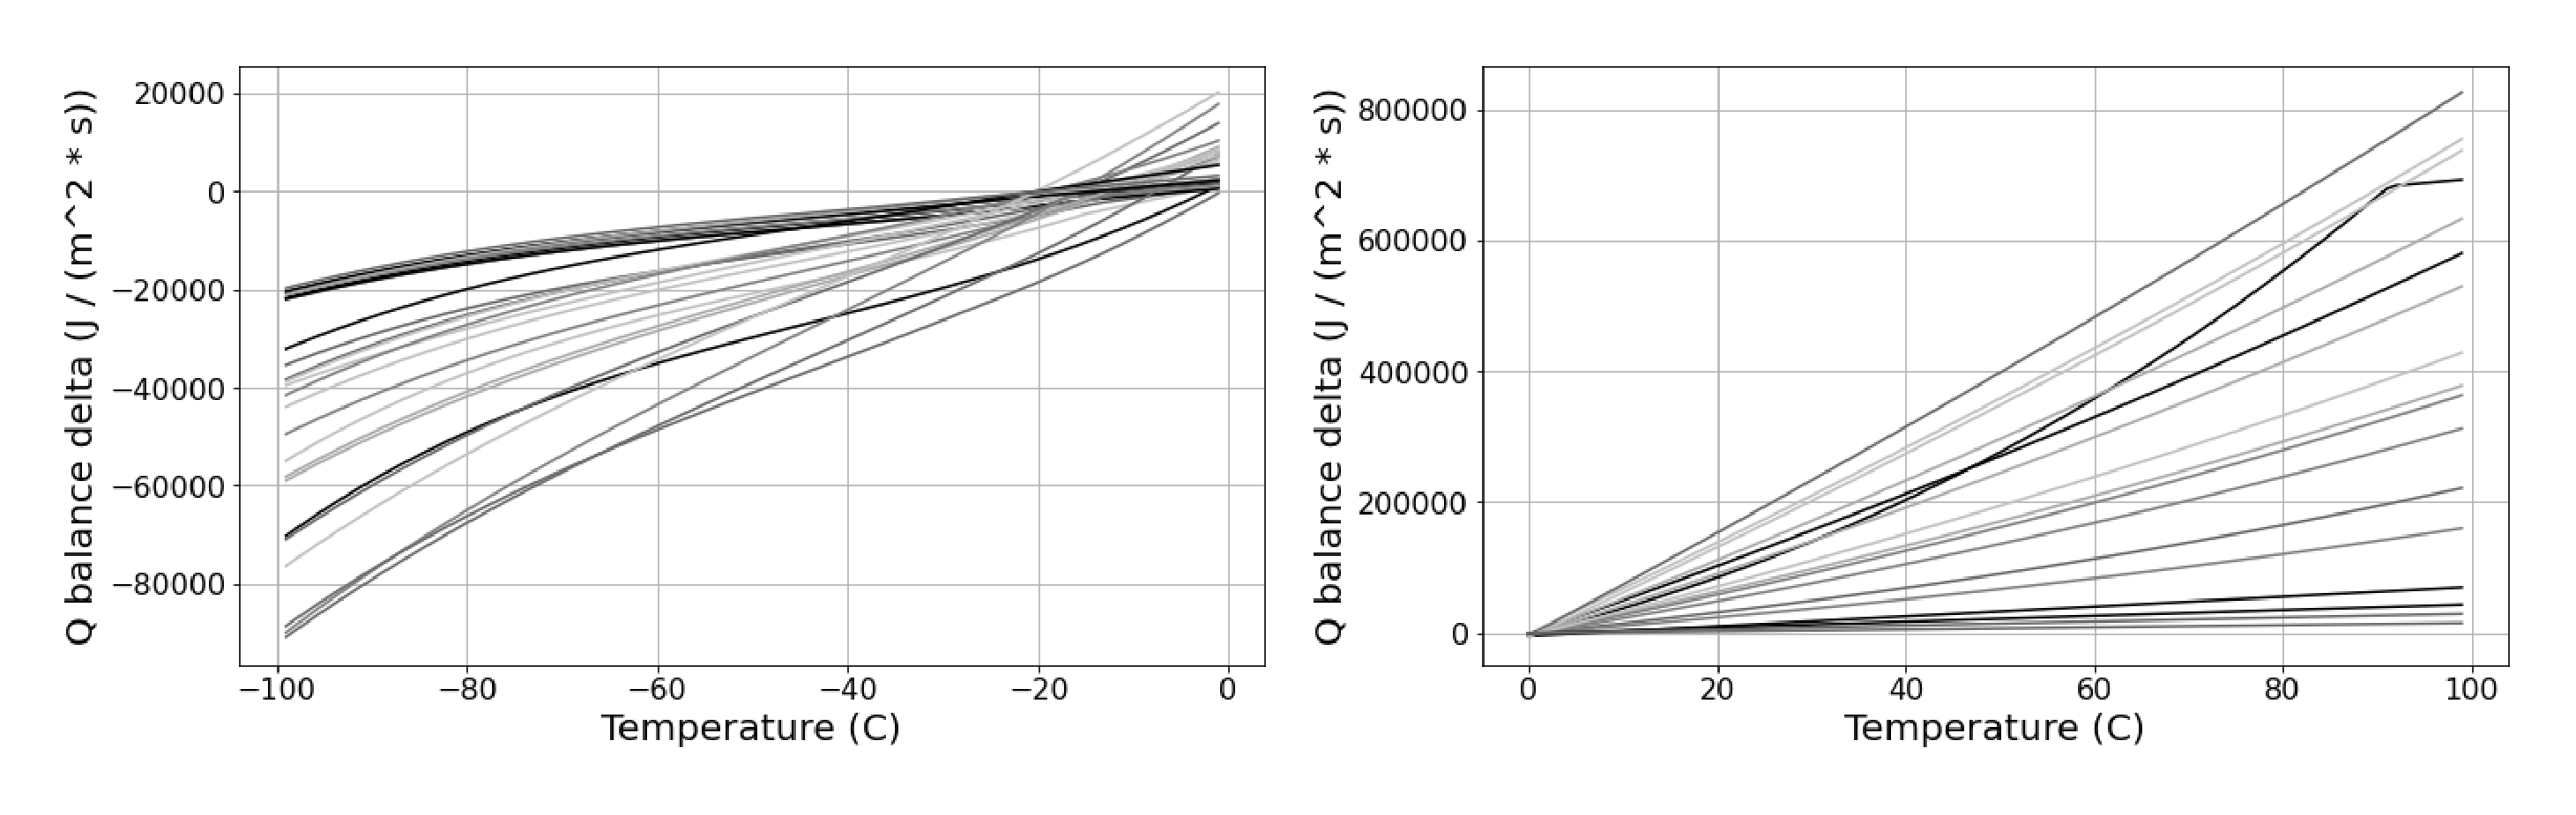
\includegraphics[width=1.0\textwidth]{pics/dq_rime_wet.pdf}
\captionstyle{normal}\caption{A family of graphs of functions for solving nonlinear equations when determining the state of cells rime ice (left) and running wet (right).}\label{fig:dq_rime_wet}
\end{figure}

\section{Methods of solving nonlinear equations}

So, we consider the solution of a nonlinear equation of the form $f(x) = 0$, obtained from a system of equations of mass and heat balance to resolve one of the states of the cell.
When choosing the optimal method for solving nonlinear equations for the problem posed, the following methods were used: bisection method, chord method, Newton's method, Brent's method.
The equations were solved in the temperature range $x \in [-100, 200]$, the condition $f(a)f(b) < 0$ was satisfied for the equations being solved.

The bisection method was considered as a reference for comparison with other methods, since it is clear that it is the slowest, but it is guaranteed to work correctly under any initial conditions and any form of the analyzed function.
In the process of solving a nonlinear equation by the bisection method, the search interval at each iteration of the solution is divided into two intervals with the same length, from which one is selected, for which the condition of the function with different signs at the ends of the interval continues to be satisfied.

The chords method is similar in meaning to the bisection method, however, at each iteration of the equation solution, the root search interval is not divided into two equal parts.
The point of dividing the search interval into two new intervals is defined as the intersection of the $OX$ axis with the geometrical segment $[(a, f (a)), (b, f (b))]$.
This method in most cases leads to a faster solution of the equation, however, profiles of functions for which the use of the chords method can lead to a catastrophic slowdown in the process of finding the root are possible.

Fig.~\ref{fig:chords-newton} shows schemes for finding the roots of a nonlinear equation using the chords methods and Newton's method.

\begin{figure}[h]
\setcaptionmargin{5mm}
\onelinecaptionstrue
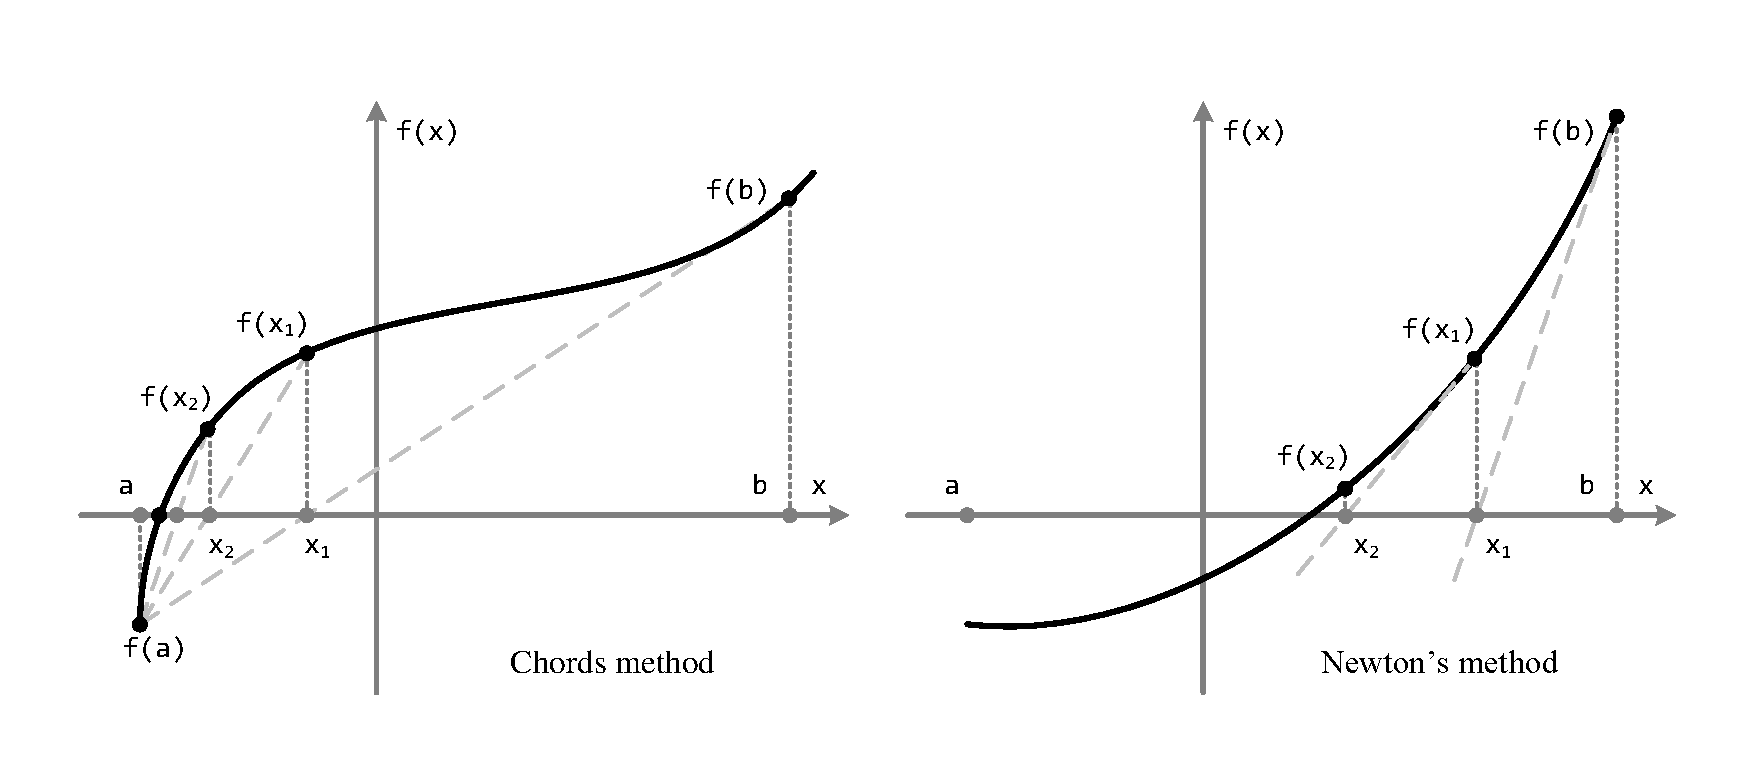
\includegraphics[width=1.0\textwidth]{pics/chords-newton.pdf}
\captionstyle{normal}\caption{Schemes for finding the root of a nonlinear equation by the chords method and Newton's method.}\label{fig:chords-newton}
\end{figure}

In Newton's method, the root of the equation is searched for starting from some point (in Fig.~\ref{fig:chords-newton} we start from point $b$).
A tangent line is drawn from this point to the intersection with the $OX$ axis (which corresponds to the calculation of the difference derivative with the required order of accuracy) at some point $x_i$, which becomes a new value - a candidate for the root of the equation.
This method is extremely effective for finding the roots of equations, represented, for example, by convex functions, but there are profiles of functions for which Newton's method is inapplicable or can be extremely slow.

Brent's method is a modified Decker's method, which, in turn, is a combination of the bisection method with the chords method.
In Decker's method, at each iteration, an attempt is made to apply the chords method step to narrow the interval for finding the root, and if the chords method cannot be applied, we use one iteration of bisection method.
In the Brent's method, a similar synthesis of the chords method and the bisection method is carried out.
This method also attempts to apply the chords method, and when the rate of contraction of the interval for root searching decreases, one iteration of the bisection method are used.
In addition, linear interpolation in the chords method has been replaced by inverse quadratic interpolation.

\section{Numerical experiments}

\begin{figure}[h!]
\setcaptionmargin{5mm}
\onelinecaptionstrue
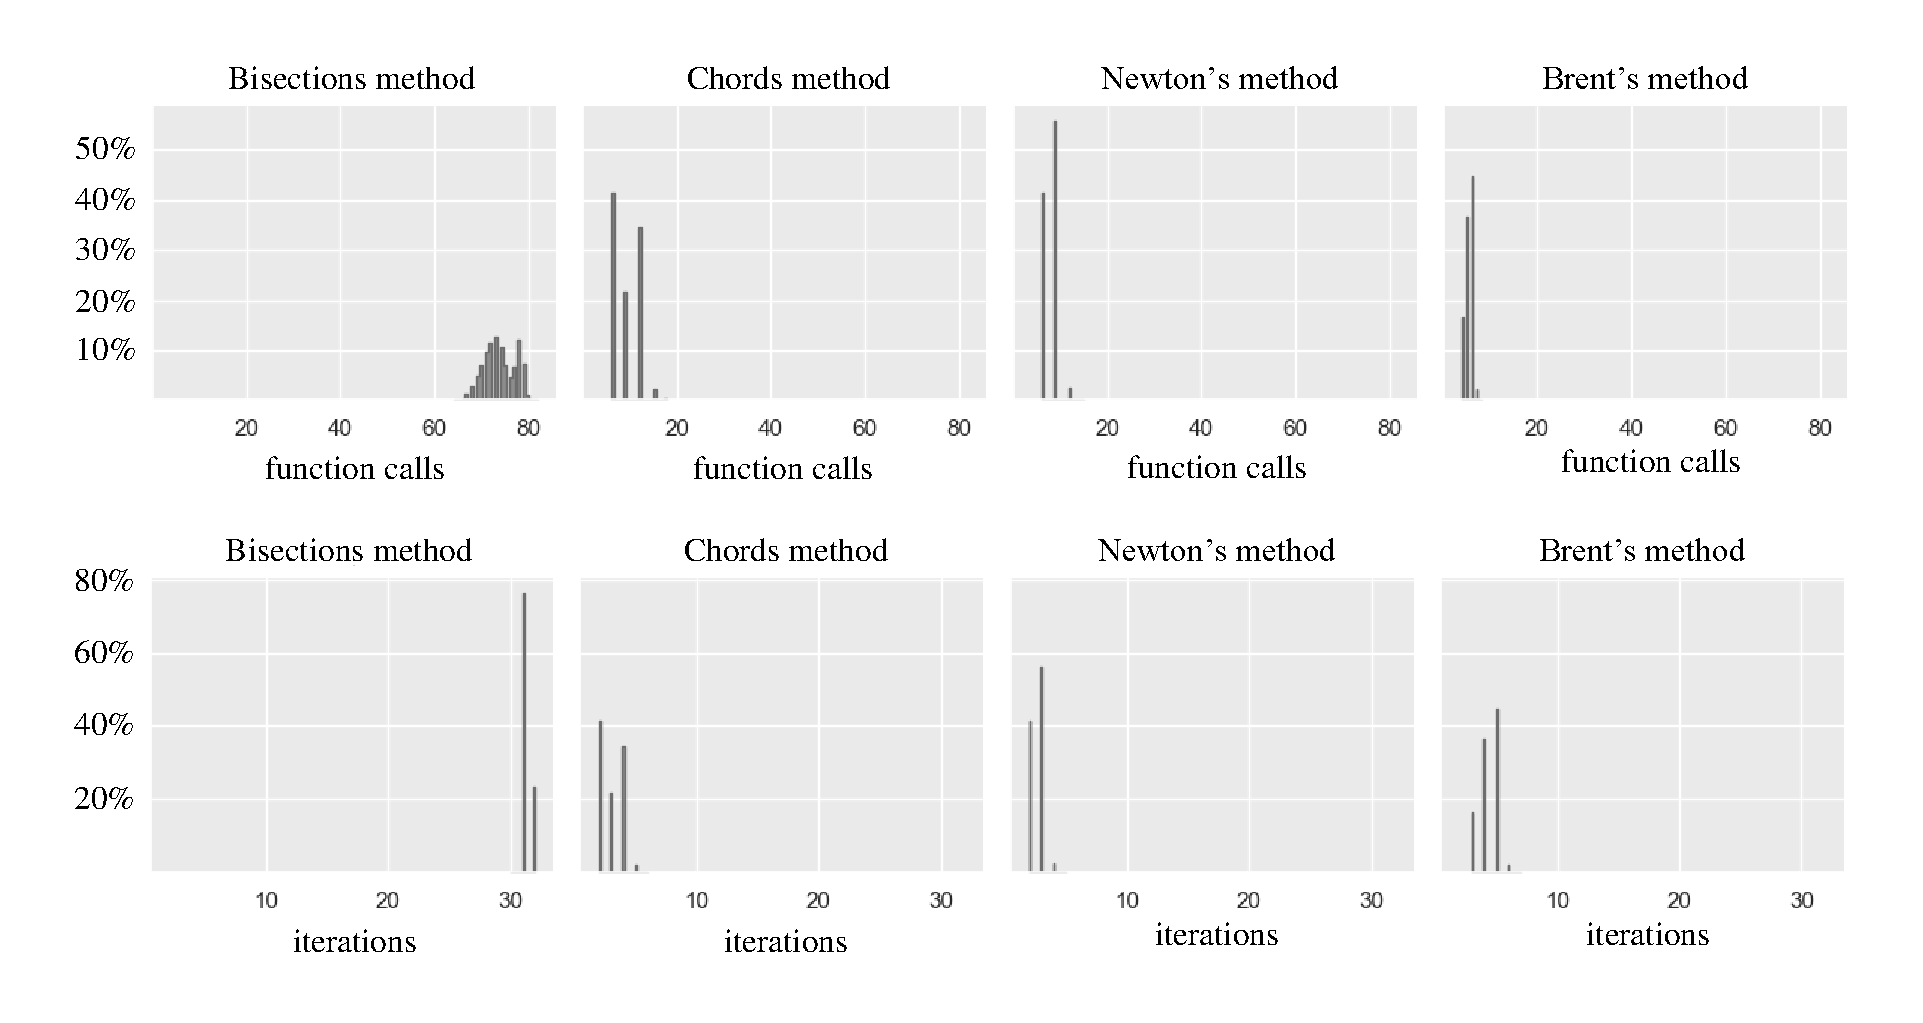
\includegraphics[width=1\textwidth]{pics/stat.pdf}
\captionstyle{normal}\caption{Statistics of the quantities of calls to the function $f(x)$ and iterations of solving a nonlinear equation.}\label{fig:stat}
\end{figure}

To analyze the use of various methods for solving nonlinear equations for launching on typical computational problems solved at different temperatures of the free stream, statistics were collected on the number of iterations of solving the equations and the total number of calls to functions $f(x)$ required to solve these equations.
Fig.~\ref{fig:stat} provides summary statistics.
Table~\ref{tab:stat} contains data on the average number of iterations and function calls when using all the described methods for solving equations.

\begin{table}[h!]
\label{tbl:supercomputers}
\setcaptionmargin{0mm}
\onelinecaptionsfalse
\captionstyle{flushleft}
\caption{Statistics on the application of various methods for solving nonlinear equations.}\label{tab:stat}
\bigskip
\begin{tabular}{|c|c|c|}
\hline
Method & Avg. func calls & Avg. iterations \\
\hline
bisections & 78,8 & 31,3 \\
\hline
chords & 11,2 & 3,7 \\
\hline
Newton's & 10,1 & 3,3 \\
\hline
Brent's & 5,5 & 4,5 \\
\hline
\end{tabular}
\label{tab:supercomputers}
\end{table}

It should be noted that the total number of calls to the function $f(x)$ during the solution of equations is the most important characteristic from the point of view of the efficiency of the method for solving a nonlinear equation, since it takes computational time.
Based on the data presented in Fig.~\ref{fig:stat} and Table~\ref{tab:stat}, we can see that Newton's method requires, on average, only 3.3 iterations to solve the considered nonlinear equations.
However, from the point of view of performance, the Brent method in the course of its work performs almost twice as few calls to the function $f(x)$, which leads to an almost twofold acceleration of the calculation speed relative to the chords method and Newton's method.

\section{Conclusion}

The work considered the formulation of the problem of calculating physical processes in the impelemtation of the shallow-water icing model.
The core of this solver is the solution of a nonlinear equation with one unknown variable.
The solution of this problem takes up the overwhelming majority of all calculations of the solver, therefore, the choice of the optimal method for solving a nonlinear equation is extremely important.
In the process of performing the research, profiles of functions were collected for which it is required to solve nonlinear equations and the following methods were analyzed on the collected data: bisection method, chords method, Newton's method and Brent's method.
From the point of view of the average number of iterations for finding the root of the equation, Newton's method turned out to be the most advantageous.
However, the total number of calls to the $f(x)$ function turned out to be lower on average when using the Brent method, which makes this method optimal for use in the shallow-water icing model solver.
\begin{acknowledgments}
The work has been done at the JSCC RAS as part of the state assignment for the topic 0580-2021-0016.
The supercomputer MVS-10P OP, located at the JSCC RAS, was used during the research.
\end{acknowledgments}

\begin{thebibliography}{99}

\bibitem{Wright}
\refitem{article}
W.~W.~Wright, P.~Struck, T.~Bartkus, G.~Addy, {\it ``Recent Advances in the LIWICE Icing Model''}, SAE Technical Paper (2015).

\bibitem{Bourgault}
\refitem{article}
Y.~Bourgault, H. Beaugendre, W. G. Habashi, {\it ``Development of a Shallow-Water Icing Model in FENSAP-ICE''}, Journal of Aircraft, Vol. 37, No. 4, 640--646 (2000).

\bibitem{Beaugendre}
\refitem{misc}
H.~Beaugendre, {\it ``A PDE-Based Approach to In-Flight Ice Accretion''}, A thesis of the degree of Doctor of Philosophy, Department of Mechanical Engineering, McGill University, Montreal, Qu\'ebec (2003).

\bibitem{Dekker}
\refitem{article}
Brent, R.P.. Finding a zero by means of successive linear interpolation. : London, 1969.

\bibitem{Brent}
\refitem{book}
Brent, R.P.. Algorithms for minimization without derivatives. : Prentice-Hall, 1973.

\bibitem{Press}
\refitem{book}
William H. Press, Saul A. Teukolsky, William T. Vetterling, and Brian P. Flannery. 2007. Numerical Recipes 3rd Edition: The Art of Scientific Computing (3rd. ed.). Cambridge University Press, USA.


\end{thebibliography}

\end{document}
